\section{Herramientas libres para simulaci�n dise�o de Hardware por descripci�n de hardware}


\subsubsection{S�ntesis, simulaci�n y verificaci�n digital}

Para la s�ntesis digital a partir de lenguajes de descripci�n de hardware se utilizan las herramientas gratuitas suministradas por los fabricantes de FPGAs, \textit{webpack} de Xilinx y \textit{Quartus} de Altera; debido a que la estructura interna de las FPGAs solo la conocen los fabricantes\footnote{Es posible obtener informaci�n valiosa de sus patentes por ejemplo: http://www.freepatentsonline.com/6301693.pdf, con este tipo de informaci�n varios proyectos buscan generar herramientas abiertas de s�ntesis}, es obligatorio utilizar sus herramientas para obtener el archivo de configuraci�n.

Para la simulaci�n de sistemas digitales que utilizan como entrada de dise�o lenguajes de descripci�n de hardware existen los simuladores \textit{ICARUS} para verilog y \textit{GHDL} para vhdl; los dos pueden ser utilizados para realizar simulaciones funcionales, post s�ntesis o post place \& route (trabajando en conjunto con las herramientas de los fabricantes) y ambos soportan el formato de salida VCD (definido junto con el lenguaje de descripci�n de hardware verilog por el est�ndar IEEE 1364-2001). Adicionalmente, estas herramientas pueden ser utilizadas en los sistemas operativos m�s utilizados.

Como herramienta de simulaci�n se utilizar� \textit{GTKWAVE}, la cual acepta como entrada archivos en formato \textit{VCD} y puede ser ejecutada en MAC, Linux y Windows. \textit{GTKWAVE} realiza un manejo adecuado de la jerarqu�a del sistema bajo an�lisis, permitiendo observar todas las se�ales de los diferentes m�dulos que componen la jerarqu�a superior, lo que es muy �til en este tipo de simulaciones; en la figura \ref{gtkwave} se puede observar una captura de esta herramienta.

  \begin{figure}[htpb]
    \begin{center} 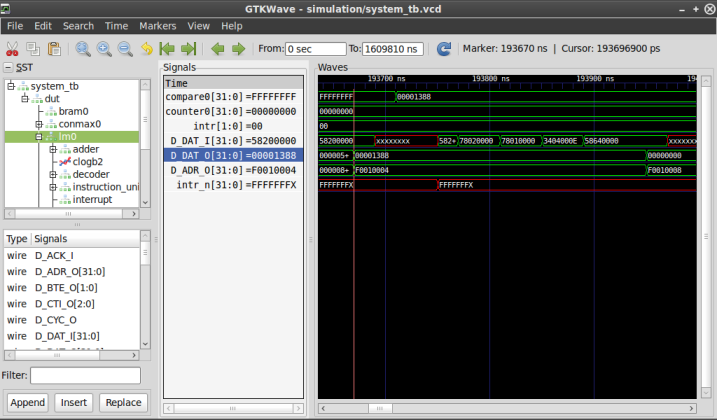
\includegraphics[scale=.7]{./anexo1/images/gtkwave.png}   \end{center}
     \caption{Visualizador de formas de onda \textit{GTKWAVE}} \label{gtkwave}
  \end{figure}

Una vez configurada la FPGA, se utiliza la herramienta \textit{URJTAG} para verificar el correcto funcionamiento del sistema implementado en la FPGA, \textit{URJTAG} proporciona una capa de abstracci�n de hardware que permite el manejo del puerto JTAG de cualquier dispositivo, proporcionando funciones de alto nivel para la aplicaci�n de las funciones JTAG (IDCODE, INTEST, EXTEST, BYPASS, SAMPLE/PRELOAD) permitiendo la aplicaci�n de vectores de prueba al n�cleo l�gico de la FPGA y la captura de la respuesta a estos est�mulos; estas pruebas se realizan a baja frecuencia. \textit{URJTAG} soporta varias interfaces f�sicas para control de las se�ales del puerto JTAG (TDI, TDO, TMS y TCK) las cuales pueden ser conectadas a diferentes puertos de un computador, o como en este caso a un puerto virtual creado en el procesador MIPS.  


\subsubsection{Herramientas para la configuraci�n de PLDs}
Aunque con la plataforma de desarrollo SIE no es necesario utilizar herramientas ni unidades de programaci�n adicionales para configurar su FPGA; el procesador de SIE ejecuta dos aplicaciones que son utilizadas para realizar esta funci�n y pueden ser ejecutadas en computadores personales: \textit{URJTAG} y \textit{XC3SPROG}, las dos funcionan de forma similar, utilizan dispositivos conectados al puerto paralelo (conexi�n directa) o USB (basados en el protocolo MPSSE del chip FT2232) del computador; para ejecutar las instrucciones extendidas de la FPGA CFG\_OUT, CFG\_IN, JSTART y JPROGRAM (hasta el momento solo han sido probadas con las FPGAs de Xilinx).

